\documentclass[unknownkeysallowed, 10pt, a4 paper, handout]{beamer}

% Custom beamer theme
\usepackage{../style/beamerthemeCustom}
\newcommand{\HRule}{\rule{\linewidth}{0.5mm}}   %FOR TITLEPAGE

\usepackage{changepage}     % adjustwidth
\usepackage{booktabs}       % \toprule, \midrule and \bottomrule
\usepackage{upquote}

\setlength\parskip{0.3cm}

\newcommand{\focus}[1]{\textbf{\textcolor{red}{#1}}}
\newcommand{\ra}{$\longrightarrow$ }
\newcommand{\lra}{$\longleftrightarrow$ }

\newcommand{\code}[1]{\colorbox{black}{\color{green}\texttt{#1}}}

% Command to create two side-by-side minipages
\newcommand{\sidebyside}[5]{
  \begin{minipage}{#1\textwidth}
    #2
  \end{minipage} #3 \begin{minipage}{#4\textwidth}
    #5
  \end{minipage}
}

\title[Linux Basic]{ICTP DP Linux Basic Course - UNIX/Linux}
\subtitle{ESP Students - First Semester}
\author[Graziano Giuliani]{Graziano Giuliani \\ \focus{ggiulian@ictp.it}}
\institute[ICTP]{The Abdus Salam International Centre for Theoretical Physics}
\date[\today]{ICTP Diploma Program \\ \today}

\begin{document}

\begin{frame}
  \titlepage
\end{frame}


\begin{frame}[label=outline]
  \frametitle{Course Outline \footnotemark}
  \framesubtitle{Daily program}
  \begin{itemize}
    \item \focus{UNIX/Linux}
      \begin{enumerate}
        \item The Shell Command Line
        \item Basic command line programs
        \item Basic file editing
      \end{enumerate}
    \item Programming on Linux
    \item Text file manipulation
    \item Basic BASH and Python
  \end{itemize}

  \vspace{6mm}

  Slides: \\ \code{http://tinyurl.com/2jsvfbd6}
  \vspace{4mm} \\
  or the \LaTeX \ source on GitHub: \\
  \code{https://github.com/graziano-giuliani/LinuxBasics}

  \footnotetext[1]{Course created in 2019 with Adriano Angelone, now LPTMC-FR}

\end{frame}


\begin{frame}[label=pdp11]
  \frametitle{The origin of UNIX}
  \framesubtitle{Operating System}
  \begin{columns}
    \begin{column}{0.50\textwidth}
      \begin{itemize}
        \item Hardware
      \begin{itemize}
        \item CPU, GPU, Motherboard, Cabling, Power
        \end{itemize}
        \item User
      \begin{itemize}
        \item Keyboard, Mouse, Monitor, etc
        \end{itemize}
        \item Software
      \begin{itemize}
        \item Application, Operating system
        \end{itemize}
      \end{itemize}
    \end{column}
    \begin{column}{0.50\textwidth}
      \begin{center}
        \includegraphics[scale=0.15]{pics/os.png}
      \end{center}
    \end{column}
  \end{columns}
  \begin{columns}
    \begin{column}{0.25\textwidth}
      \begin{center}
        \includegraphics[scale=1.15]{pics/pdp11.jpg} \\
      \end{center}
    \end{column}
    \begin{column}{0.75\textwidth}
      \begin{itemize}
            \item 1969 - Multi-Tasking Multi-User Unix AT\&T
        \item 1991 - Free Unix OS for Intel X86 (Linux)
      \end{itemize}
    \end{column}
  \end{columns}
  \begin{flushleft}
    \tiny{By Peter Hamer: Ken Thompson (sitting) and Dennis Ritchie \\
          at PDP-11 Magnus Manske, CC BY-SA 2.0}
  \end{flushleft}
\end{frame}


\begin{frame}[label=unix]{UNIX Philosophy}
  \frametitle{The UNIX Philosophy}
  \framesubtitle{Why UNIX is such a good idea}
  \begin{enumerate}
    \item Make each program do one thing well. %To do a new job, build
      % afresh rather than complicate old programs by adding new "features".
    \item Expect the output of every program to become the input to another.
      %, as yet unknown, program. Don't clutter output with extraneous
      % information. Avoid stringently columnar or binary input formats.
      % Don't insist on interactive input.
    % \item Design and build software, even operating systems, to be tried
      % early, ideally within weeks. Don't hesitate to throw away the clumsy
      % parts and rebuild them.
    % \item Use tools in preference to unskilled help to lighten a programming
      % task, even if you have to detour to build the tools and expect to
      % throw some of them out after you've finished using them.
    % \item Write programs to handle text streams, because that is a
      % universal interface.
    \item Purpose of computation is data transformation
  \end{enumerate}
  \vfill
  \emph{$\dots$ at its heart is the idea that the power of a system comes
  more from the relationships among programs than from the programs themselves.
  Many UNIX programs do quite trivial things in isolation, but, combined with
  other programs, become general and useful tools. \dots}
  \newline
  \begin{flushright}
  \tiny{The UNIX Programming Environment, Brian Kernighan and Rob Pike, 1984}
  \end{flushright}
\end{frame}


\begin{frame}[label=os]
  \frametitle{The Linux Revolution}
  \framesubtitle{Why a free OS is a good idea}
  \begin{center}
    \includegraphics[scale=0.5]{pics/linux-first-announcement-email.png}
  \end{center}
\end{frame}


\begin{frame}[label=gnu]
  \frametitle{The Free Software Movement}
  \framesubtitle{Free Software as in Freedom}
  \begin{columns}[T]
    \begin{column}{.68\textwidth}
      \begin{block}{The Freedom to}
        \begin{itemize}
          \item run the program as you wish, for any purpose
          \item study how the program works, and change it as you wish
          \item redistribute copies so you can help others
          \item distribute copies of your modified versions to others
        \end{itemize}
      \end{block}
    \end{column}
    \hfill
    \begin{column}{.32\textwidth}
      \begin{flushright}
        \includegraphics[scale=0.35]{pics/rms1.png} \\
      \end{flushright}
    \end{column}
  \end{columns}
  \begin{center}
    \includegraphics[scale=0.25]{pics/GPL.png}
  \end{center}
\end{frame}


\begin{frame}[label=architecture]
  \frametitle{Linux architecture}
  \framesubtitle{Linux is the kernel and we do not hate it!}
  \begin{columns}[T]
    \begin{column}{.23\textwidth}
      \vspace{7mm}
      \includegraphics[scale=0.5]{pics/UNIX-HATERS_Handbook_cover_ISBN_1-56884-203-1.png}
    \end{column}
    \begin{column}{.73\textwidth}
      \begin{itemize}
      \item The Linux kernel is a program that loads all the other programs and
        supervise the resources allocated to each one of them, providing
        locking and I/O services.
      \item The system services \emph{(daemons)} are programs running on the
        system and providing facilities that allow or enhance access to system
        resources.
      \item User programs are controlled interactively or through batch job
        submission system by physical users concurrently accessing system
        resources through a multi tasking sharing of the CPU(s).
    \end{itemize}
    \end{column}
  \end{columns}
\end{frame}


\begin{frame}[c]
  \begin{center}
    \frametitle{The Command Line}
    \framesubtitle{The old terminal}

    \sidebyside{0.54}{
      \focus{Command Line Interface (CLI)}:\\
             programmable, steep(-ish) learning curve
    }{\hfill}{0.41}{
      \includegraphics[width=\textwidth]{pics/cli.png}
    }

    \sidebyside{0.54}{
      \focus{Graphical User Interfaces (GUI)}:\\
      intuitive, difficult to program
    }{\hfill}{0.41}{
      \includegraphics[width=\textwidth]{pics/gui.png}
    }

    \vspace{-2mm}

    We're here to learn (mostly) how to use CLI:\\
    headaches at first, more productivity in the end

  \end{center}
\end{frame}


\begin{frame}[label=login]
  \frametitle{Authentication}
  \framesubtitle{Multi-User}
  To support multiple users, Linux require authentication before
  authorizing the user programs to allocate system resources.
  \begin{columns}[T]
    \begin{column}{.23\textwidth}
      \begin{center}
        \includegraphics[scale=0.25]{pics/locks.png}
      \end{center}
    \end{column}
    \hfill
    \begin{column}{.66\textwidth}
    \vspace{5mm}
    \small{
      \begin{itemize}
        \item \textbf{Authentication}: The user is authenticated with
          username/password challenge by a login program.
        \item \textbf{Authorization}: The system creates an environment
          by providing the set of system resources the user may access 
        \item \textbf{Allocation}: The user access the resources by
          running programs through a command interpreter.
      \end{itemize}
      }
    \end{column}
  \end{columns}
\end{frame}


\begin{frame}[label=shell]
  \frametitle{The command shell}
  \framesubtitle{How it works}
  The SHELL is a text based command interpreter
  \begin{columns}[T]
    \begin{column}{.60\textwidth}
    \begin{center}
    \begin{block}
    \small{
      \begin{itemize}
        \item waits for the user command input showing up a prompt 
        \item controls the user environment through variables
        \item executes user commands managing the input, output
                 and error streams
      \end{itemize}
      }
    \end{block}
    \end{center}
    \end{column}
    \hfill
    \begin{column}{.40\textwidth}
      \begin{center}
        \includegraphics[scale=0.4]{pics/vt100.png}
      \end{center}
    \end{column}
  \end{columns}
  \begin{center}
    There is not just a single shell program!
  \end{center}
\end{frame}

\begin{frame}[label=program]
  \frametitle{Linux Program}
  \framesubtitle{Running a program in the CLI}
  The User must type in a command line at the CLI prompt
  \vspace{5mm} \\
  \begin{columns}[T]
    \begin{column}{.39\textwidth}
      \includegraphics[scale=0.13]{pics/running.jpg}
    \end{column}
    \begin{column}{.61\textwidth}
      A typical UNIX command line contains:
      \begin{block}{}
        \begin{itemize}
          \item The name of the program executable
          \item The options modifying the execution
            \begin{itemize}
              \item short format: -f
              \item long format: -\ -\ a\_longer\_string
            \end{itemize}
          \item The argument or list of arguments
        \end{itemize}
      \end{block}
      \begin{alertblock}{}
        Options and arguments may have convenient defaults!
      \end{alertblock}
    \end{column}
  \end{columns}
  As an example, these are valid syntax for command lines:
  \vspace{3mm} \\
  \code{ls -l Documents} \\
  \code{cp --force theorem.tex Documents}
\end{frame}


\begin{frame}[c]
  \begin{block}{}
    \frametitle{Files and directories}
    \framesubtitle{Exploring the filesystem}

    \focus{Directories contain files, files contain information}
    \vspace{3mm} \\

    \code{/} is the filesystem root directory
    \vspace{-3mm} \\
    \begin{center}
      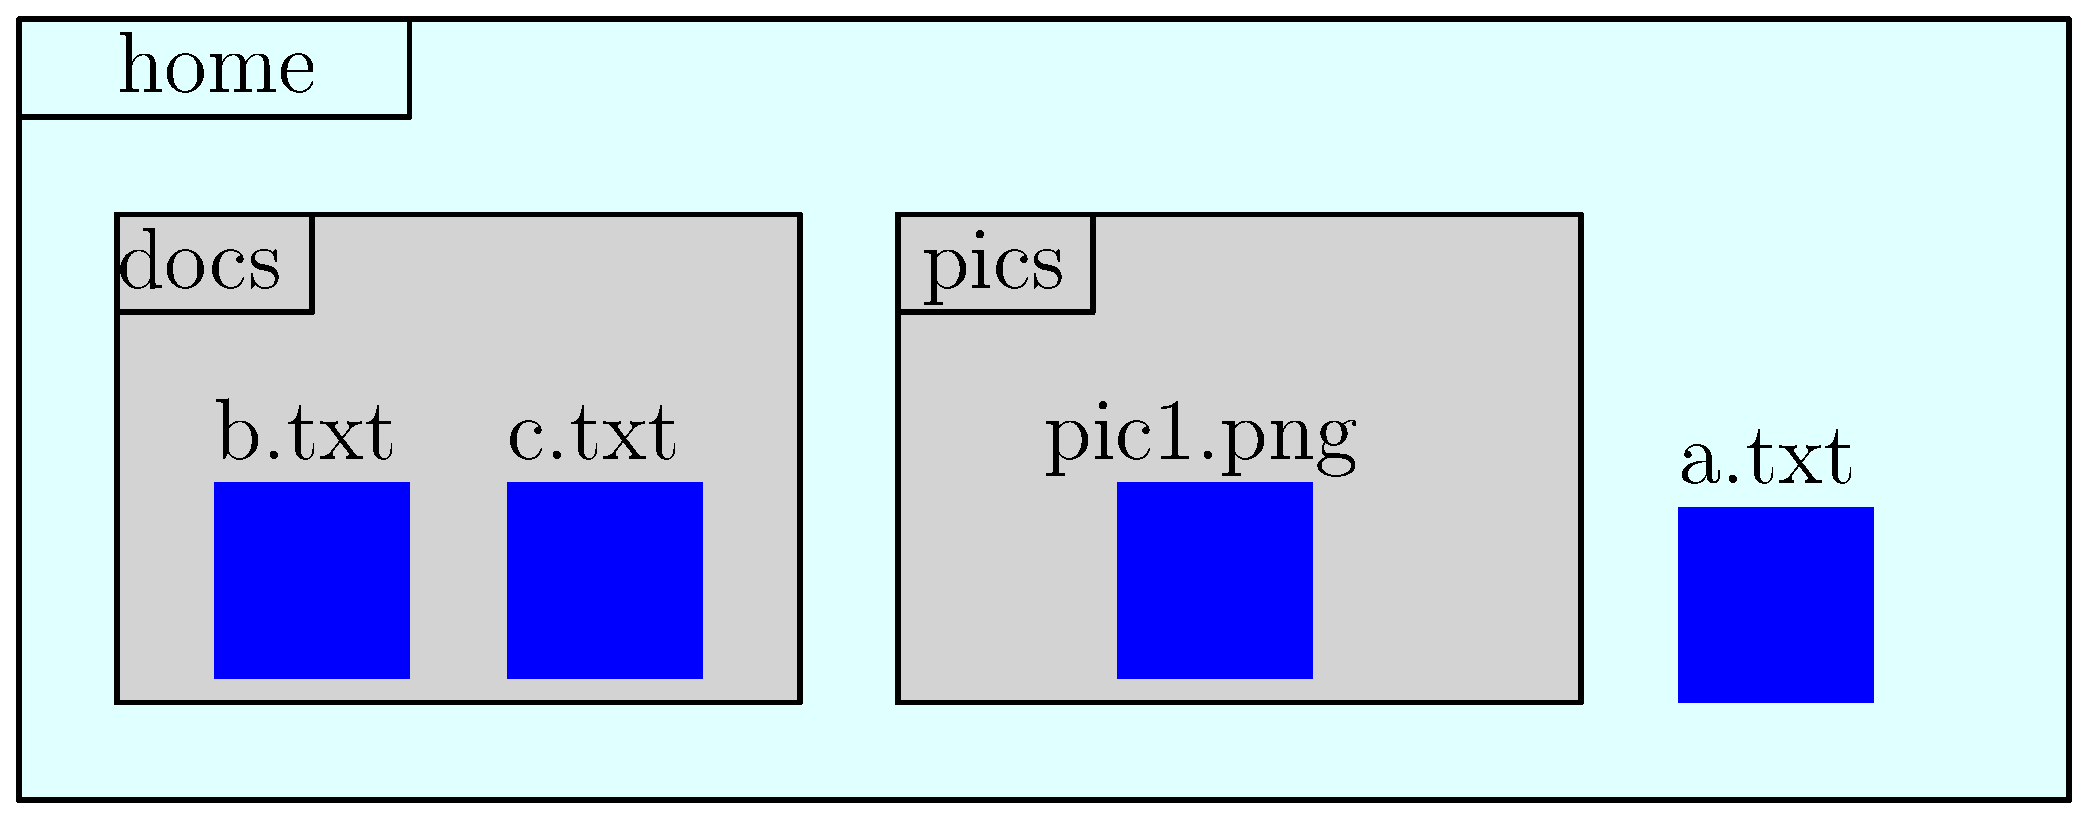
\includegraphics[width=0.90\textwidth]{pics/filesystem.eps}
    \end{center}

    Directories in a path are separated by \code{/}
    \vspace{3mm} \\
    Files and directories have a \focus{full path} in the filesystem: \\
    \code{/home/docs/c.txt} \hspace{4mm}FQP: Fully Qualified Path
  \end{block}
\end{frame}


\begin{frame}[label=filesystem]
  \frametitle{The file system}
  \framesubtitle{Filesystem Hierarchy Standard (FHS)}
  All files and directories appear under the root directory \code{/},
  even if they are stored on different physical or virtual devices.
  \begin{columns}[T]
    \begin{column}{.23\textwidth}
      \includegraphics[scale=0.23]{pics/fs.png}
    \end{column}
    \hfill
    \begin{column}{.73\textwidth}
      \small{
      \begin{itemize}
	\item \code{bin} : binaries, contains system executables
        \item \code{lib} : libraries, contains shared or static pieces of
          code which are used by running executables or to create executables
        \item \code{tmp} : system or user temporary files
        \item \code{etc} : configuration files
	\item \code{home} : user files (one directory per user)
      \end{itemize}
    }
    \begin{alertblock}{Home directory}
      \code{.} : the current directory\\
      \code{..} : the parent of the current directory\\
      \code{/home/\{user\}} is the default CWD
    \end{alertblock}
    \end{column}
  \end{columns}
\end{frame}


\begin{frame}[c]
  \frametitle{Commands}
  \framesubtitle{Path finding}

  Let us try to run the basic programs to navigate the Filesystem:
  \begin{exampleblock}{Print the current directory FQP}
    \code{pwd}
  \end{exampleblock}

  \code{pwd} prints the \focus{fully qualified path} of the current directory
  \begin{exampleblock}{}
    \begin{center}
    \includegraphics[width=0.40\textwidth]{pics/pwd.png}
    \end{center}
  \end{exampleblock}

  In commands, you use by default the \focus{relative path} respect to
  the \focus{CWD}: \\
  \code{a.txt} without a path is a file in the current working directory

  \begin{alertblock}{Have you noticed?}
    \code{pwd} does not require options or arguments\\
    \code{CWD} stands for Current Working Directory
  \end{alertblock}{}
\end{frame}


\begin{frame}[c]
  \frametitle{Commands}
  \framesubtitle{Moving around}

  \begin{exampleblock}{List a file or the files in a directory}
    \code{ls \{directory or file\}} \\
    \includegraphics[scale=0.20]{pics/ls.png}
  \end{exampleblock}

  \begin{exampleblock}{Change the working directory}
    \code{cd \{directory\}} \\
    \includegraphics[scale=0.20]{pics/cd.png}
  \end{exampleblock}

  \begin{alertblock}{Have you noticed? Default arguments and options!}
     \code{ls} without arguments list the content of the \focus{CWD}\\    
     \code{cd} without arguments change the CWD to the user home directory
  \end{alertblock}

\end{frame}


\begin{frame}[c]
  \frametitle{Commands}
  \framesubtitle{Creating new filesystem objects}

  \begin{exampleblock}{Create new directories}
    \code{mkdir <directories>}\\
    \includegraphics[scale=0.20]{pics/mkdir.png}
  \end{exampleblock}

  \begin{exampleblock}{Create new (empty) text files}
    \code{touch <filenames>}\\
    \includegraphics[scale=0.20]{pics/touch.png}
  \end{exampleblock}

  \begin{alertblock}{Have you noticed?}
    A plural is specified above. Guess what it means?
  \end{alertblock}
\end{frame}

\begin{frame}[c]
  \frametitle{Commands}
  \framesubtitle{Removing existing filesystem objects}

  \begin{exampleblock}{removes files and directories}
    \code{rm <filenames>}\\
    \code{rm -r <directories>} \\
    \includegraphics[scale=0.20]{pics/rm.png}
  \end{exampleblock}

  \begin{alertblock}{ATTENTION!}
    The remove operation cannot be undone. There is no Trash directory.\\
    Be careful, especially in using the recursive \code{-r} option!!!
  \end{alertblock}
\end{frame}


\begin{frame}[c]
  \frametitle{Manual}
  \framesubtitle{What are all the possible options?}

  \begin{exampleblock}{Reading the manual pages}
    In CLI mode, you can access the manual page for each command in text
    format. \\
    \code{man <command>}
  \end{exampleblock}

  \begin{alertblock}{ATTENTION!}
    The formatting of the manual page on the text window is a complex
    operation and depends on the available lines/rows of the terminal.
    To be compatible with old terminals, the best window size for the
    man program is at \focus{80rows x 24 lines}. 
  \end{alertblock}
\end{frame}


\begin{frame}[c]
  \frametitle{Exercise I}
  \framesubtitle{cd, mkdir, touch, rm}
  \begin{block}{}
    Using the commands we have seen, create the below directories and files,\\
    and then remove them all (\focus{after carefully checking}):
    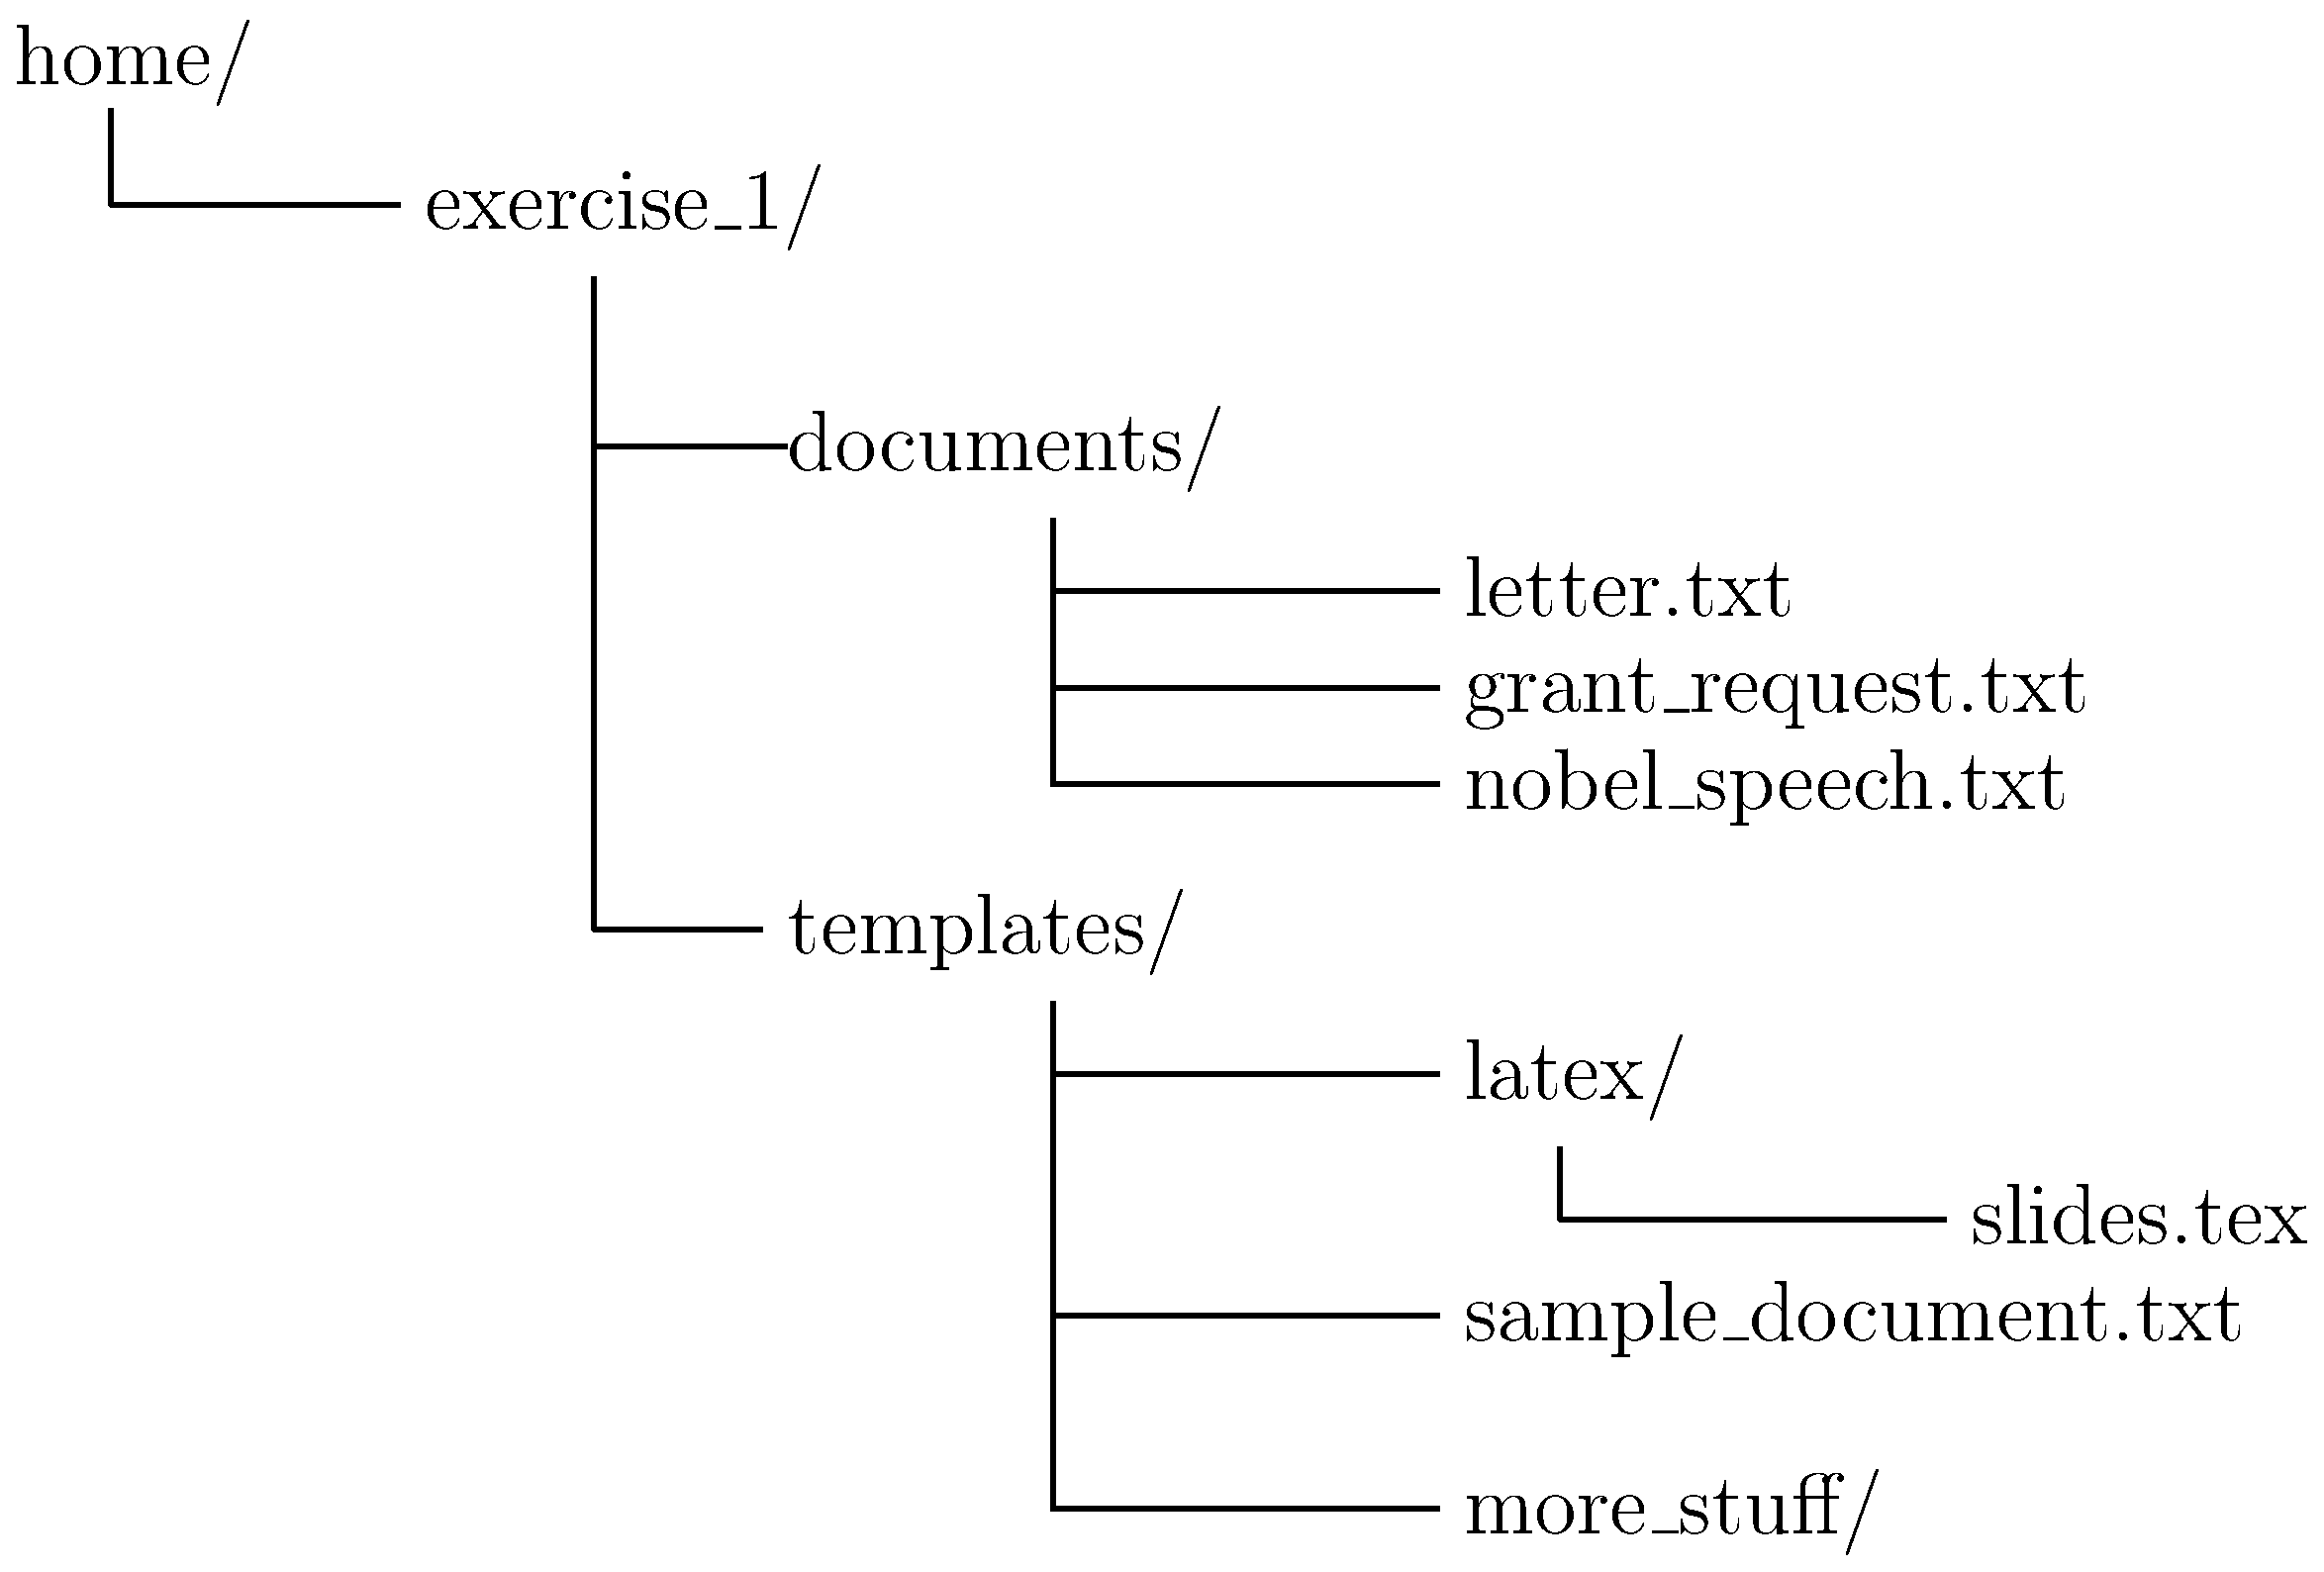
\includegraphics[scale=0.17]{pics/exercise_1.eps}
  \end{block}
  \begin{alertblock}{How to check?}
    \code{ictp-install tree}\\
    \code{tree home}
  \end{alertblock}
\end{frame}


\begin{frame}[c]
  \frametitle{Solution to Exercise I}
  \begin{block}{Creation part}
  \small{
  \code{cd} \\
  \code{mkdir -p home/exercise\_1/documents} \\
  \code{mkdir -p home/exercise\_1/templates/\{latex,more\_stuff\}} \\
  \code{cd home/exercise\_1/documents} \\
  \code{touch letter.txt grant\_request.txt nobel\_speech.txt} \\
  \code{cd ../templates} \\
  \code{touch latex/slides.tex sample\_document.txt} \\
  \code{cd}
  }
  \end{block}
  \begin{block}{Removal part}
  \small{
  \code{cd} \\
  \code{rm -r home}
  }
  \end{block}
\end{frame}


\begin{frame}
  \frametitle{Commands}
  \framesubtitle{Moving and copying files}

  \begin{exampleblock}{Copy an object to another location}
  \code{cp <old\_path> <new\_path>} \\
  \includegraphics[scale=0.20]{pics/cp_1.png}
  \includegraphics[scale=0.20]{pics/cp_2.png}
  \end{exampleblock}

  \begin{alertblock}{Attention! \code{<new\_path>} is overwritten and lost!}
  Suggestion: use \code{cp -i}\\
  \code{cp -r}: copy entire directories
  \end{alertblock}

  \begin{exampleblock}{Move an object to another location}
  \code{mv <old\_path> <new\_path>}\\
  Same syntax as \code{cp}, \code{old\_path} is removed after copy.
  \end{exampleblock}
\end{frame}


\begin{frame}
  \frametitle{Commands}
  \framesubtitle{Finding and listing files}

  \begin{exampleblock}{Recursively searches files in a directory}
  \code{find <directory> <options>}
  \end{exampleblock}

  \sidebyside{0.52}{
     \begin{itemize}
      \item \code{-name}:\\
        specify file name (no paths here)
      \item \code{-path}:\\
        specify (part of) the file path
      \item \code{-printf \%\{format\}}:\\
        print details of the items found
      \item \code{-delete}:\\
        deletes the files found
    \end{itemize}
  }{\hfill}{0.45}{
    \begin{center}
      \includegraphics[width=1.00\textwidth]{pics/find.png}
    \end{center}
  }

  \begin{alertblock}{You can use wildcards}
  \code{*} can replace any character (more in the future)
  \end{alertblock}
\end{frame}


\begin{frame}
  \frametitle{Exercise II}
  \framesubtitle{cp, mv, find}
  \begin{block}{}
    Using the commands you know, create these directories and files,\\
    copying and moving files as shown:

    \begin{center}
      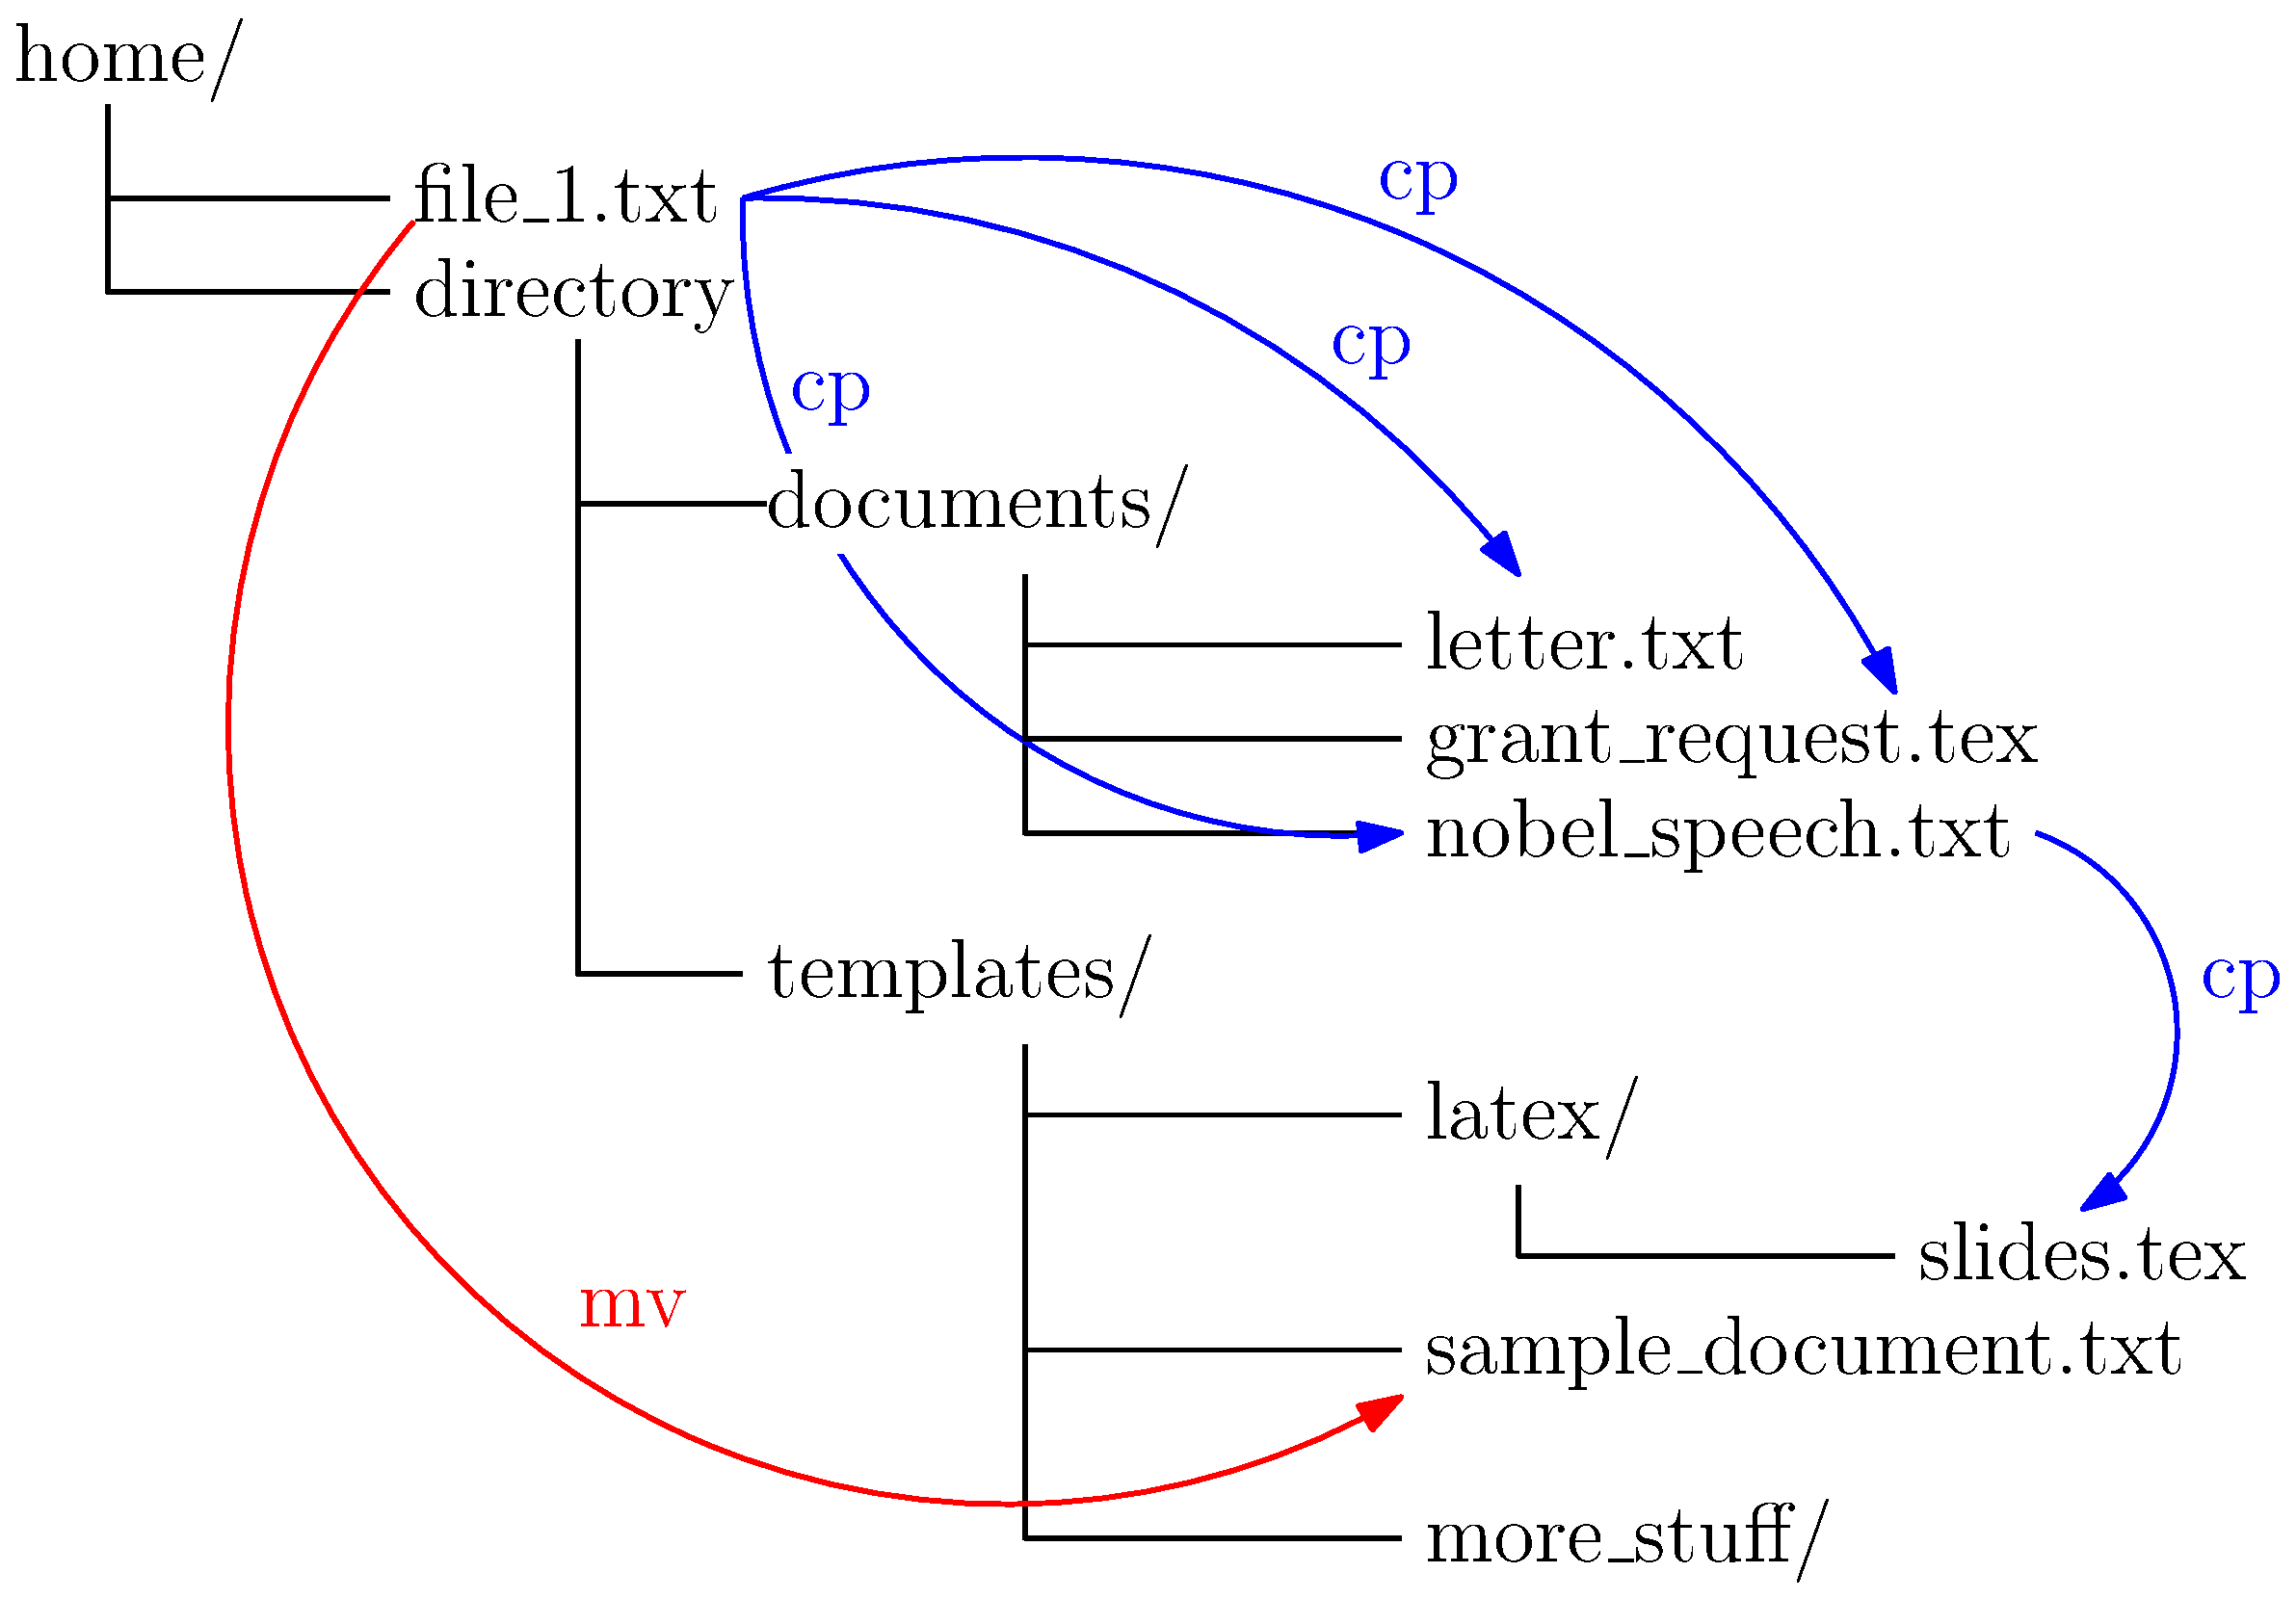
\includegraphics[scale=0.15]{pics/ex_2.eps}
    \end{center}

    Then, using \code{find}, show the location of all \code{.tex} files
  \end{block}
  \begin{alertblock}{}
    Be careful with the order of the operations!
  \end{alertblock}
\end{frame}


\begin{frame}
  \frametitle{Text file editors}
  \framesubtitle{Edit text files from the command line}

  \begin{block}{Install some programs to edit text file}
  \code{ictp-install emacs nano ne tilde vim} \\
  \end{block}

  \begin{alertblock}{There is NO default editor program}
  I have selected the editors in alphabetic order.\\
  You need to try all of them and select the one you like more!
  \end{alertblock}

  \begin{exampleblock}{}
    \begin{itemize}
      \item vim is powerful but arcane
      \item emacs is even more powerful and arcane
      \item nano is simple and CTRL based
      \item ne is simple and ESC based
      \item tilde is simple and ALT based
    \end{itemize}
  \end{exampleblock}
\end{frame}


\begin{frame}[fragile=singleslide]
  \frametitle{Exercise III}
  \framesubtitle{Text editing}
  \begin{exampleblock}{}
    Using the above command line text editors, create and save a text file
    \code{first.csv} with the following content:
   \begin{verbatim}
# Year Month Day Precipitation
2000,06,01,23.0
2000,06,02,3.0
2000,06,03,7.0
2000,06,04,0.0
2000,06,05,2.0
2000,06,06,0.0
2000,06,07,0.0
2000,06,08,0.0
2000,06,09,1.0
2000,06,10,0.0
    \end{verbatim}
  \end{exampleblock}
  \begin{alertblock}{ATTENTION!}
    Keep the file! We will use it tomorrow!
  \end{alertblock}
\end{frame}

\end{document}

%vim: tabstop=8 expandtab shiftwidth=2 softtabstop=2 spell spelllang=en_GB
